\section{Proposed Method - For High Utilization Tasks}
\revise{We define candidates for collapse as a pair of nodes that share the same cache block, and other conditions. Identifying potential candidates for collapse is discussed in the following/previous section. For this section, we assume that the potential candidates are at the same depth from the start node and they are not dependent on each other. } 

In a federated scheduler, a high utilization task $T_i$ is allocated $m_i$ dedicated cores, given by Equation (\ref{eq:m}), where no other tasks can execute. In this environment, collapsing two nodes in the DAG of high utilization task $T_i$ is beneficial to the federated scheduler if the collapse decreases the required number of cores. Formally, consider the number of cores dedicated to a task ${T_i}$ before any two nodes are collapsed as ${m_i}$ as calculated by Equation~\ref{eq:m}. The number of cores dedicated to ${T_i}$ after collapse are denoted ${\hat{m}_i}$.

\textbf{Beneficial Collapse}: Collapsing two nodes of a task ${T_i}$ is \emph{beneficial} if ${\hat{m}_i \le m_i}$.

\revise{We need more supportive definitions before the proof, \\ 
  1 inter-thread cache benefit for two collapsed nodes ${v_j}$ and ${v_k}$ for the same executable object \\
  2 max extension of paths by ${\iota_j}$ for two collapsed nodes ${v_j}$ and ${v_k}$. \\
  3 "resulting path" -- the single path that results from ${v_j}$ and ${v_k}$ being collapsed from separate paths
  }

In Theorem~\ref{thrm:conditional-collapse}, we derive a sufficient condition to determine if collapsing two nodes is beneficial. The proof is divided into four sections. Each is related to the impact of collapse upon the longest path through the DAG of ${T_i}$.

%\newtheorem{theorem}{Theorem}
\begin{theorem}[Conditional Collapse]\label{thrm:conditional-collapse} For a DAG task ${T_i}$, collapsing two \textbf{candidate} nodes ${v_j, v_k \in V_i}$ (which refer to the same executable object) is \textbf{beneficial} if:

    \begin{equation}\label{eq:cond}
        1 + \frac{\gamma_j}{\iota_j} > \frac{C_i  - L_i }{D_i - L_i}
    \end{equation}
\end{theorem}
\begin{proof}
A direct proof supports the theorem, it is divided into four cases 1.) collapsing two nodes off the critical path where the critical path length is not affected 2.) collapsing two nodes with exactly one lies on the critical path 3.) collapsing two nodes where both lie on the critical path 4.) collapsing two nodes off the critical path, which creates a new critical path length.

\emph{Case 1.} Collapsing two nodes off the critical path with no impact to the critical path length. Since ${v_j}$ and ${v_k}$ refer to the same executable object ${\iota_j = \iota_k}$ and ${\gamma_j = \gamma_k}$. Collapsing ${v_j}$ and ${v_k}$ in the graph serializes the execution of threads on the same processor. This decreases the execution time ${v_k}$ (or ${v_j}$) due to the inter-thread cache benefit; which is quantified as ${2 \cdot \iota_j + \gamma_j}$. This increases the path(s) of ${v_j}$ and ${v_k}$ by at most ${\iota_j}$. 
\end{proof}
%\end{theorem}
%\blacksquare

Collapsing two nodes of DAG tasks always results in a decrease in the worst-case execution time of the task by $\mathbb{B}$. Nevertheless, collapsing two nodes of DAG tasks may increase the critical path by $\mathbb{I}$, may increase the critical path by a value less than $\mathbb{I}$ but greater than $0$, or may not change the critical path length value. For example, Fig.~\ref{fig:c1}, Fig~\ref{fig:c2}, and Fig.~\ref{fig:c3} show the three cases, i.e., case 1 when there is no change in critical path length, case 2 when the critical path length increases by $\mathbb{I}$, and case 3 when the critical path length increases by a values greater than $0$ but less than $\mathbb{I}$.

\begin{figure}
  \centering
  \begin{subfigure}[b]{0.4\textwidth}{
      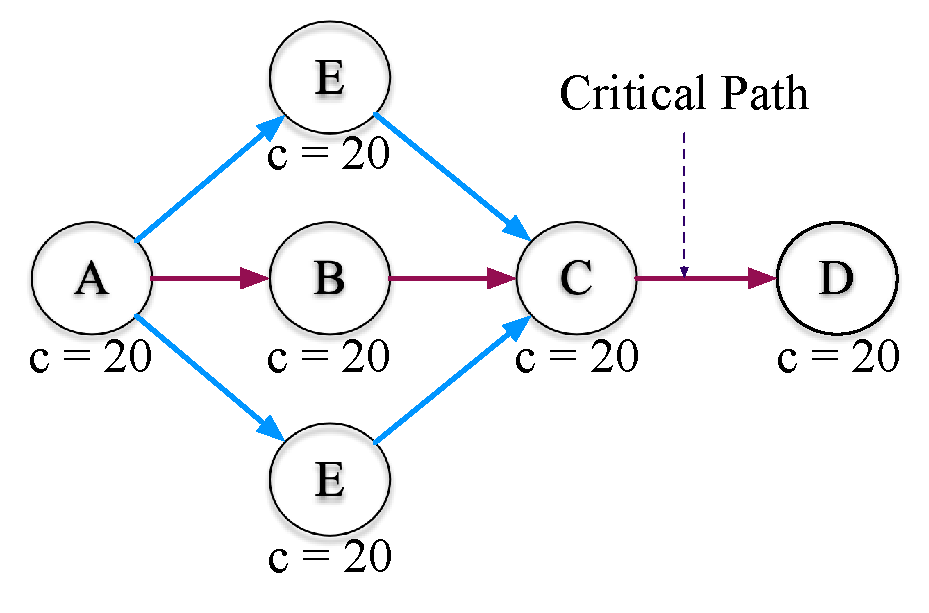
\includegraphics[width=\textwidth]{c1before}
      \caption{Before Collapse}
      \label{fig:c1before}
    }
  \end{subfigure}~
  \begin{subfigure}[b]{0.4\textwidth}{
      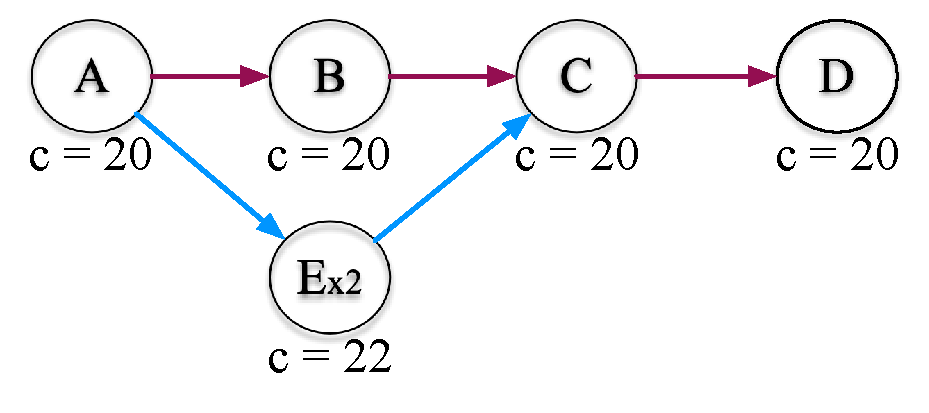
\includegraphics[width=\textwidth]{c1after}
      \caption{After Collapse}
      \label{fig:c1after}
    }
  \end{subfigure}
  \caption{Case 1:  No change in the critical path length}
  \label{fig:c1}
\end{figure}

%% \begin{figure}
%% 	\subfigure[Before collapse]{
%% 		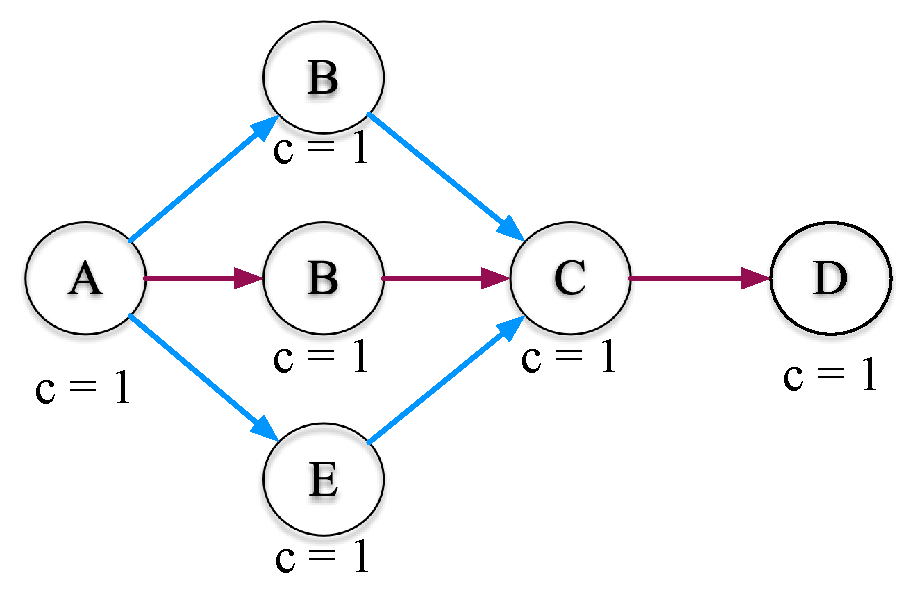
\includegraphics[width=0.22\textwidth]{figs/c2before.eps}
%% 		\label{fig:c2before}
%% 	}
%% 	\subfigure[After collapse]{
%% 		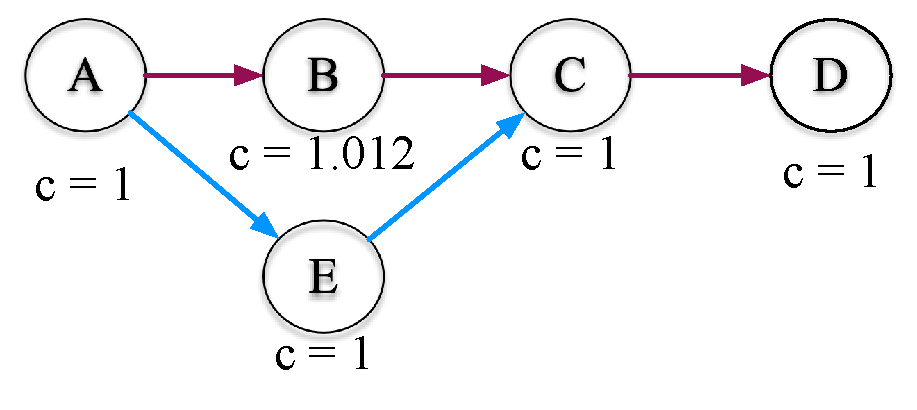
\includegraphics[width=0.22\textwidth]{figs/c2after.eps}
%% 		\label{fig:c2after}
%% 	}
%% 	\caption{Case 2:  Critical path length increases by $\mathbb{I}$}
%% 	\label{fig:c2}
%% \end{figure}

%% \begin{figure}
%% 	\subfigure[Before collapse]{
%% 		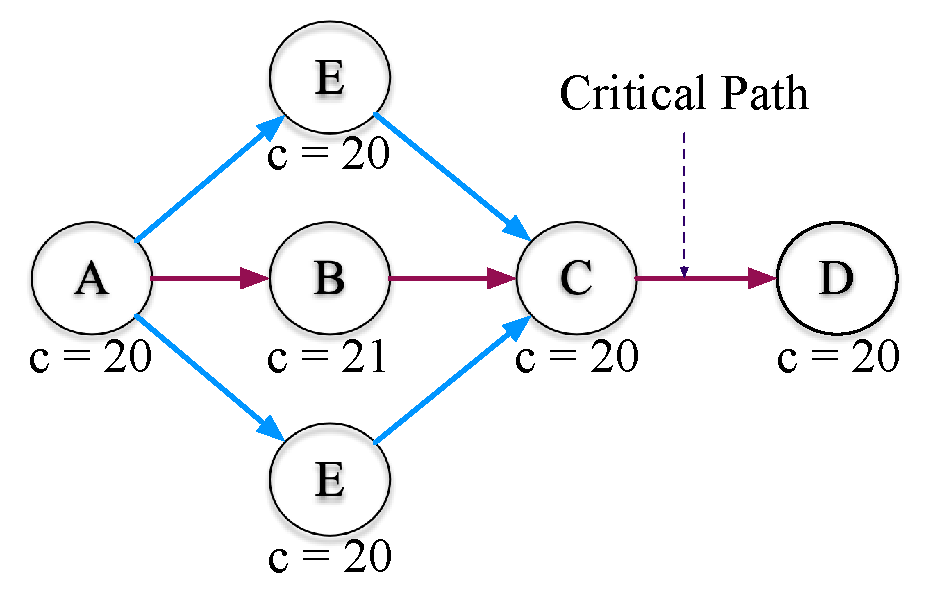
\includegraphics[width=0.22\textwidth]{figs/c3before.eps}
%% 		\label{fig:c3before}
%% 	}
%% 	\subfigure[After collapse]{
%% 		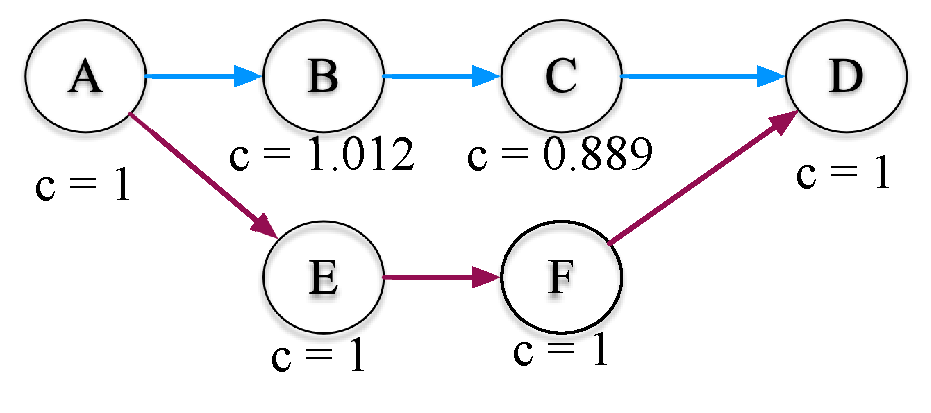
\includegraphics[width=0.22\textwidth]{figs/c3after.eps}
%% 		\label{fig:c3after}
%% 	}
%% 	\caption{Case 3:  Critical path length increases by a value less than $\mathbb{I}$}
%% 	\label{fig:c3}
%% \end{figure}


In case 1, there is no change in the critical path length but the worst case execution decreases by $\mathbb{B}$,thus the required number of cores after collapse, given by $\frac{C_i - \mathbb{B} - L_i}{D_i - L_i}$, is less than the required number of cores before collapse, given by $\frac{C_i - L_i}{D_i - L_i}$  (since $\frac{C_i - \mathbb{B} - L_i}{D_i - L_i} < \frac{C_i - L_i}{D_i - L_i}$). Therefore, any two nodes that fall under case 1 can be considered for collapse. 

In case 2, the task $T_i$ saves $\mathbb{B}$ units of worst-case execution time however it increases the critical path length by $\mathbb{I}$. Similarly, in case 3, the task $T_i$ saves $\mathbb{B}$ units of worst-case execution time however it increases the critical path length by at most $\mathbb{I}$. To derive a sufficient condition, we consider the upper bound on the increase in critical path length, i.e., $\mathbb{I}$ as the increase in critical path length. Thus, under case 2 and 3, a task receives a saving of $\mathbb{B}$ in worst-case execution time but spends $\mathbb{I}$ on the critical path. In case 2 and 3, collapsing two nodes can decrease the number of cores if Equation (\ref{eq:cond}) holds.

\begin{equation} \label{eq:cond} 1 + \frac{\mathbb{B}}{\mathbb{I}} > \frac{C_i  - L_i }{D_i - L_i} \end{equation}

To prove this, let us assume the Equation (\ref{eq:inequality}) is true.
\begin{equation} \label{eq:inequality} \frac{C_i - \mathbb{B} - (L_i + \mathbb{I})}{D - (L_i + \mathbb{I})}  < \frac{C_i  - L_i }{D_i - L_i} \end{equation}
Then by algebraic simplification, the following inequality is also true.
$$ - ( \mathbb{B} + \mathbb{I}) (D_i - L_i)  < -\mathbb{I}(C_i  - L_i )$$
Further simplification shows that the following inequality is also true.
$$ 1 + \frac{\mathbb{B}}{\mathbb{I}} > \frac{C_i  - L_i }{D_i - L_i}$$
Since the obtain result is obtained from algebraic simplification of Equation (ref{eq:inequality}), we can conclude that if Equation (\ref{eq:cond}) is true then Equation (\ref{eq:inequality}) is also true.
